


\chapter{The Ancestral Recombination Graph (ARG)}
{\bf Object}: for simulating genealogical histories of sample sequences subject to recombination. \\
{\bf Difficulties}: Recombination events are difficult to detect.

$N$ denotes the number of individuals, and there are $2N$ gene copies at each locus (diploid individuals). At one particular locus, for $2N$ gernations, mutation parameter is $\theta=\lim_{N\rightarrow\infty}4Nu$ and the recombination parameter is $\rho=\lim_{N\rightarrow\infty}4Nr$, where $u$ and $r$ are the probability of mutation and recombination per locus per generation.

\section{The expected value and the variance for segregating site.}
Segregating site (\begin{CJK*}{UTF8}{gbsn}多态性位点\end{CJK*}): A DNA base-pair position at which polymorphism is observed in a population \citep{Kimura1971}. Note that the number of segregating sites is the total number of mutation in the history of a sample.

Under the infinite site model, we assume that mutations always occur on the new site; and the number of mutations is a Poisson random variable with the mean of $\frac{\theta}{2}t$ \citep{Wakeley2008}, where $\theta$ is the mutation rate per generation.

Let $K$ denote the number of mutations over 1 unit of coalescent time, $K$ is a Poisson random variable with rate of $\frac{\theta}{2}t$, where time $t=1$. For a Poisson random variable $K$, we have
\begin{equation}
\EE[K]=\var[K]=\frac{\theta}{2}.\label{eq:mean_var_of_K}
\end{equation}

Let $T_i$ be the time in the hisotry of the smaple during which there are exactly $i$ ancestral lineages, then the total length of all the branches is $T_{total}=\sum^n_{i=2}iT_i$. Under the Kingman coalescent, $T_i$ is an exponential random variale with rate $\binom{i}{2}$, thus $\EE[T_i]=\frac{2}{i(i-1)}$. Therefore, \citet{Wakeley2008} Equation (3.23) gives the expected value of $T_{total}$ as 
\begin{equation}
\EE[T_{total}]=\sum^n_{i=2}i \EE[T_i]=2\sum^{n-1}_{i=1}\frac{1}{i}\label{Wakeley2008:eq:3.23}.
\end{equation}
Variance of $T_i$ is $\binom{i}{2}^{-2}$, and 
\begin{equation}
\var[T_{total}]=\sum^n_{i=2}i^2\var[T_i]=4\sum^{n-1}_{i=1}\frac{1}{i^2}.\label{Wakeley2008:eq:3.25}
\end{equation}

Let $S$ denote the number of segregating site in a sample of size $n$. The number of mutations in the history of a sample is equal to the number of mutations per generation summed over the total length, i.e. $S=K\cdot T_{total}$. The formula of calculating the probability of $S$ equal to a particular number $k$ can be found in \citet{Wakeley2008} Equation (4.3).

The expected value and variance of $S$ are first given by \cite{Watterson1975}, we are using notations and formulas from \citet{Wakeley2008}, Equation (4.7) and (4.8) (refer \citet{Wakeley2008} Equations (2.32) and (2.33) for why). Use Equations \eqref{eq:mean_var_of_K}, \eqref{Wakeley2008:eq:3.23} and \eqref{Wakeley2008:eq:3.25}, we have

\begin{equation}
\EE[S]=\EE[K]\EE[T_{total}]=\frac{\theta}{2}\left(2\sum_{i=1}^{n-1}\frac{1}{i}\right)=\theta\sum_{i=1}^{n-1}\frac{1}{i},\label{wakeley2008:eq:4.7}
\end{equation}
\begin{align}%or \begin{multiline}
\var[S]&=\var[K]\EE[T_{total}]+\EE[K]^2\var[T_{total}]\notag\\
&=\frac{\theta}{2}\left(2\sum_{i=1}^{n-1}\frac{1}{i}\right)+ \left(\frac{\theta}{2}\right)^2\left(4\sum_{i=1}^{n-1}\frac{1}{i^2}\right)\notag \\
&=\theta\sum_{i=1}^{n-1}\frac{1}{i}+\theta^2\sum_{i=1}^{n-1}\frac{1}{i^2},\label{wakeley2008:eq:4.8}
\end{align}
The sequence of $\sum_{i=1}^{n-1}\frac{1}{i}$ does not converge, but diverges slowly.

In \citet{Watterson1975}, these expressions are given for a dipoid locus, by let $n=2$ (see Equation (1.10), $K_2$ is defined at the top of page 258 \citep{Watterson1975}):

\begin{align}
\EE[S]&=\theta,\label{Watterson1975:1.10:exp}\\ 
\var[S]&=\theta+\theta^2.\label{Watterson1975:1.10:var}
\end{align}

{\color{red}{\bf Questions:}
\begin{enumerate}
\item When there is free recombination between sites, $S$ follows a Poisson distribution, so $\var[S]=\EE[S]=\theta$??? With some  recombination and zero recombination, the variance is bigger than the mean. Overdispersion???
\end{enumerate}
} 

\section{Number of mutations and recombinations in recombination models}
\subsection{Mutations in recombination models (summary of \citet{Hudson1983TPB})}
Under the standard Kingman coalescent process, all the sites in the sequence share the same genealogy \citep{Wakeley2008} page 94.

\citet{Hudson1983TPB} suggested that to first build the recombination model for a two loci model, then for an $m$-locus model. Put $m$-locus sequence together. Each locus is treated as a subloci of the whole sequence, sequence on each subloci follows the infinite-site model. When $m\rightarrow\infty$, we then have the recombination model for infinite site model. So, in fact it is double infinite here. One of the key message is that {\bf recombination does not occur within subloci, but between two adjacent subloci with rate $r/(m-1)$.}

\subsection{Two loci model} Let $n$ be the sample size. According to Equation \eqref{wakeley2008:eq:4.7}, for loci 1 and 2, the expected values of the segregating sites are $\EE[S_1]=\theta_1\sum_{i=1}^{n-1}\frac{1}{i}$ and $\EE[S_2]=\theta_2\sum_{i=1}^{n-1}\frac{1}{i}$. For the expected value of the total number of the segregating site $S$, it is 
$$
\EE[S]=\EE[S_1+S_2]=\EE[S_1]+\EE[S_2]=\theta\sum_{i=1}^{n-1}\frac{1}{i},
$$
where $\theta=\theta_1+\theta_2$.
The variance is given by 
$$\var[S]=\var[S_1]+\var[S_2]+\cov[S_1,S_2],$$
where $\var[S_1]=\theta_1+\theta_1^2$ (by Equation \eqref{Watterson1975:1.10:var}) and $\cov[S_1,S_2]=\theta_1\theta_2\frac{\rho+18}{\rho^2+13\rho+18}$ given by \citet{Griffiths1981} Equation (6.2), and \citet{Wakeley2008} Equation (7.16). The derivation of $\cov[S_1,S_2]$ relies on $\cov[T_1,T_2]$\citet{Wakeley2008} Equation (7.17), which is expanded in section 7.2.4, from Equations (7.26) to (7.30), and refer to Table 7.1 and Figure 7.7.


\subsection{$m$-loci model}
Consider the $m$-loci model rather than the two loci model, we have the expected value of the segregating site as 
\begin{equation}
\EE[S]=\theta\sum_{i=1}^{n-1}\frac{1}{i},\label{eqn:EE:seg_num}
\end{equation} where $\theta_j=\frac{\theta}{m}$ for all $j\in \{1,2,\dots,m\}$.
And the variance is 
\begin{align}
\var[S]&=\sum^m_{j=1}[S_j]+\sum_{k\neq j}\cov[S_j,S_k],\notag\\
&=\sum^m_{j=1}[S_j]+2\sum^{m-1}_{j=1}\sum^m_{k=j+1}\cov[S_j,S_k],\notag\\
&=\theta+\theta^2\frac{2}{\rho^2}\int^\rho_0(\rho-x)f_2(x)dx,\label{eqn:var:seg_num}
\end{align}
where 
\begin{equation}
f_2(x)=\frac{x+18}{x^2+13x+18}.\label{f2x}
\end{equation} {\color{red} Don't really understand how yet...}


{\color{red} When to use the approximation of the variance? \citet{Hudson1983TPB} Equations (3) and (7).}

\subsection{Number of recombination events in recombination models (summary of \citet{Hudson1985})}

Let $R$ be the nuber of recombination events in the ancestry of a sample in the infinite-sites $m\rightarrow\infty$ model (similar setting as the previous section and \citet{Hudson1983TPB}). The expected value and the variance of $R$ are as the following:
\begin{align}
\EE[R]&=\rho \sum^{n-1}_{i=1}\frac{1}{i},\label{eqn:EE:recomb_num}\\
\var[R]&=\rho\sum^{n-1}_{i=1}\frac{1}{i}+2\int^\rho_0(\rho-x)f_n(x)dx.\label{eqn:var:recomb_num}
\end{align} 
These two expression are very similar to the expected value and the variance of the number of segregating sites in Equations \eqref{eqn:EE:seg_num} and \eqref{eqn:var:seg_num}, by simply replacing $\theta$ with $\rho$. Reason is that because the subloci on the genome are numbered from left to right. If we let $R_j$ be the number of recombination events that occur immediately to the right of subloci $j$ (that is, between subloci $j$ and subloci $j+1$), for $1\leq j\leq m-1$, we have $R=\sum^{m-1}_{j=1}R_j$. Then $T_{total,j}$ represents the total opportunity for recombination at subloci $j$ and is identical to the total opportunity for mutation at subloci $j$.

However, note that $f_n(x)$ in Equation \eqref{eqn:var:recomb_num}, when $n=2$, $f_2(x)$ is the same as Equation \eqref{f2x}, when $n\geq 3$, $f_n(x)\approx\frac{n}{2x(n-1)}$ \citet{Hudson1985}.




%\section{The ancestral selection graph (\citep{Wakeley2008} section 7.2)} Natural selection ??\\ \citep{Wakeley2008} section 5.4 \\ diploid Wright-Fisher mode




\section{Griffiths' \citep{Griffiths1991,Griffiths1997ARG} ARG models}

\subsection{ARG in Two locus model (summary of \citet{Griffiths1991})}
Two locus model(\begin{CJK*}{UTF8}{gbsn}双基因座模型\end{CJK*})
\citep{Griffiths1981}

\citet{Griffiths1981} page 103

In a single-locus model the waiting time $T_n$ until there is a common ancestor of $n$ genes is a sum of mutually independent exponential random variables with rates $n(n-1)/2, \dots, 1$. The density of $T_n$ (which is $T_{MRCA}$, denotes the time that from the bottom of the tree to the root.) is known \citep{Tavare1984} and 
$$\EE(T_n)=2(1-\frac{1}{n}).$$ As $n\to \infty$ the distribution of $T_n$ converges to a proper distribution.

\begin{proof}
$T_n=\sum^n_{r=2}T_r$, where $T_r$ denote the time interval that $r$ lineages coalesce into $r-1$ lineages. 
\end{proof}

\begin{theorem}
Let $W_n$ be the waiting tim e until there is a common ancestor of sample of $n$ genes in the two-locus ancestral graph, then
$$\EE(W_n)=2\rho^{-1}\int^1_{0} \frac{1-v^{n-1}}{1-v}(e^{\rho(1-v)}-1)dv.$$
\end{theorem}




Consider the number of lineages as a birth and death process with rates $\lambda_k=k\rho/2$ {\color{red} Note this rate and the rates that involves $\rho/2$ later.}, $\mu_k=\binom{k}{2}$, $k=1,2,\dots$, as shown in Figure \ref{fig:bd_process}

\begin{figure}[htp]
\centering
\begin{tikzpicture}[thick,scale=2, node distance = 2.5cm]
\node (A){1};
%\node [below of=A,node distance=1cm]{$2/n$};
\node  (B)[right of=A]{2};
%\node [below of=B,node distance=1cm]{$4/n$};
\node   (C)[right of=B]{3};
%\node [below of=C,node distance=1cm]{$6/n$};
\node  (CD)[right of=C, node distance = 1cm]{\dots};
\node  (D)[right of=CD, node distance = 1cm]{$k$};
%\node [below of=D,node distance=1cm]{$8/n$};
\node  (E)[right of=D]{$k+1$};
\node  (F)[right of=E, node distance = 1cm]{\dots};
% \path[->](A.east) edge[out=315,in=225] (A.west);
%\draw[->](A.east)arc(400:140:.2);
%\draw[->](B.east)arc(400:140:.2);
%\draw[->](C.east)arc(400:140:.2);
%\draw[->](D.east)arc(400:140:.2);
\draw [->,out=45,in=135](A.north)to node[above]{$\lambda_1=\rho/2$}(B.north);
\draw [->,out=-135,in=-45](B.south)to node[below]{$\mu_2=1$}(A.south);
\draw [->,out=45,in=135](B.north)to node[above]{$\lambda_2=\rho$}(C.north);
\draw [->,out=-135,in=-45](C.south)to node[below]{$\mu_3=3$}(B.south);
%\draw [->,out=45,in=135](C.north)to node[above]{$1-6/n$}(D.north);
%\draw [->,out=-135,in=-45](D.south)to node[below]{$1-2/n$}(C.south);
\draw [->,out=45,in=135](D.north)to node[above]{$\lambda_k=k\rho/2$}(E.north);
\draw [->,out=-135,in=-45](E.south)to node[below]{$\mu_{k+1}=\binom{k+1}{2}$}(D.south);
\end{tikzpicture}
\caption{}\label{fig:bd_process}
\end{figure}

\subsection{ARG in the infinite sites model (summary of \citet{Griffiths1997ARG})}
{\color{red}
\paragraph{Gerton:}The original model for sequences evolving under the coalescent with recombination, proceeding back in time.  Mathematically clean, but as an algorithm very slow.
}

\subsection{Simulating new genealogy}
Propose the branch length

Since the waiting time for $k$ lineages to coalesce to $k-1$ lineages or to split into to $k+1$ lineages is a exponential random variable with rate $\lambda_k$ or $\mu_k$ resepectively, where $\lambda_k=k\rho/2$,$\mu_k=\binom{k}{2}$. Therefore, we can propose the branch length $l$ from exponential distribution with rate $\lambda_k+\mu_k$. Then we generate a random number between zero and one, if the number is less than $\frac{\lambda_k}{\lambda_k+\mu_k}$, two random lineages coaleces; otherwise, we introduce a new lineage, which is splits off from one of the existing lineages.

\section{MS \citep{Hudson2002ms}}
{\color{red}
\paragraph{Gerton:}Implements the ARG \citep{Griffiths1997ARG}, with some additions, and speeds up the algorithm by pruning the process as far as possible 
}

Examples: (refer to the Hudson MS manual {\bf Crossing over} section)
\begin{enumerate}
\item ~\\
\begin{tabular}{lp{11cm}}
{\tt ms} & calling function\\
5& number of individuals in each replicate\\
2& number of replicates, therefore, the output has two trees, it's divided into two blocks\\
-T& option to simulate genealogies\\
| tail -n +4 & remove the first 4 lines of the ouput\\
| grep -v // & remove the // signs in the output
\end{tabular}
\begin{verbatim}
$ ms 5 2 -T | tail -n +4 | grep -v // > treefile_no_recomb
$ cat treefile_no_recomb 
(5:0.544,((3:0.010,4:0.010):0.314,(1:0.088,2:0.088):0.237):0.219);

((5:0.039,(2:0.009,3:0.009):0.030):1.437,(1:0.279,4:0.279):1.197);
\end{verbatim}



\item ~\\
\begin{tabular}{lp{11cm}}
-r 3.0 & define the recombination rate $\rho=4Nr$, where $r$ is the recombination rate on each subloci\\
1000 & the number of sites between which recombination can occur\\
{\color{red} [ ]} & {\color{red} [The number in the brakets] indicates the number of nucleotides that share the same genealogy. The sum of the numbers in the brackets should be equal to the number of sites between which recombination can occur.} \\
\end{tabular}
\begin{verbatim}
$ ms 5 2 -T -r 3.0 1000 | tail -n +4 | grep -v // > treefile_recomb
$ cat treefile_recomb 
[307](5:0.647,((3:0.010,4:0.010):0.044,(1:0.032,2:0.032):0.022):0.593);
[13](5:1.204,((3:0.010,4:0.010):0.044,(1:0.032,2:0.032):0.022):1.150);
[328](5:0.402,((3:0.010,4:0.010):0.044,(1:0.032,2:0.032):0.022):0.348);
[313](5:0.360,((3:0.010,4:0.010):0.044,(1:0.032,2:0.032):0.022):0.306);
[18](5:0.360,((3:0.010,4:0.010):0.044,(1:0.032,2:0.032):0.022):0.306);
[20](5:0.430,((3:0.010,4:0.010):0.044,(1:0.032,2:0.032):0.022):0.376);
[1](5:0.707,((3:0.010,4:0.010):0.044,(1:0.032,2:0.032):0.022):0.653);

[76]((1:0.065,4:0.065):1.335,(5:0.494,(2:0.316,3:0.316):0.178):0.906);
[17]((1:0.117,4:0.117):1.283,(5:0.494,(2:0.316,3:0.316):0.178):0.906);
[140]((1:0.117,4:0.117):1.161,(5:0.494,(2:0.316,3:0.316):0.178):0.784);
[163]((1:0.117,4:0.117):1.161,(5:0.494,(2:0.016,3:0.016):0.478):0.784);
[70]((1:0.117,4:0.117):1.161,(5:0.494,(2:0.016,3:0.016):0.478):0.784);
[385]((1:0.117,4:0.117):1.161,(5:0.494,(2:0.016,3:0.016):0.478):0.784);
[40]((1:0.117,4:0.117):1.669,(5:0.494,(2:0.016,3:0.016):0.478):1.292);
[109]((1:0.117,4:0.117):0.669,(5:0.494,(2:0.016,3:0.016):0.478):0.292);
\end{verbatim}


\item ~\\
\begin{tabular}{lp{11cm}}
-t 10.04 & mutation rate $\theta=4N_0\mu$ where $N_0$ is the diploid population size and where $\mu$ is the neutral
mutation rate for the entire locus. 

\end{tabular}
\begin{verbatim}
$ ms 5 2 -T -t 10.04 -r 3.0 1000
ms 5 2 -T -t 10.04 -r 3.0 1000 
46742 40304 29623

//
[476](5:0.296,(3:0.160,(2:0.066,(1:0.064,4:0.064):0.002):0.094):0.136);
[178](5:1.316,(3:0.160,(2:0.066,(1:0.064,4:0.064):0.002):0.094):1.156);
[138](5:0.990,(3:0.160,(2:0.066,(1:0.064,4:0.064):0.002):0.094):0.830);
[54]((3:0.160,(1:0.064,4:0.064):0.096):0.830,(2:0.196,5:0.196):0.793);
[55]((3:0.160,(1:0.064,4:0.064):0.096):0.905,(2:0.196,5:0.196):0.869);
[22]((3:0.160,(1:0.064,4:0.064):0.096):1.156,(2:0.196,5:0.196):1.120);
[77]((3:0.160,(1:0.064,4:0.064):0.096):1.491,(2:0.196,5:0.196):1.454);
segsites: 20
positions: 0.0492 0.1514 0.1846 0.3859 0.4799 0.5490 0.5697 0.5734 0.5778 
0.6400 0.7447 0.7558 0.7818 0.8144 0.8332 0.8568 0.8592 0.8813 0.9505 0.9667 
11110000010110110100
11100000010101001011
01100000010100110100
11100000010100110100
00001111101001001011

//
[470]((4:0.072,(2:0.033,3:0.033):0.039):0.581,(1:0.392,5:0.392):0.261);
[333]((4:0.072,(2:0.033,3:0.033):0.039):0.581,(1:0.326,5:0.326):0.326);
[115]((4:0.072,(2:0.033,3:0.033):0.039):0.581,(1:0.643,5:0.643):0.010);
[82]((4:0.072,(2:0.033,3:0.033):0.039):0.581,(1:0.366,5:0.366):0.287);
segsites: 21
positions: 0.0193 0.0369 0.0600 0.1218 0.1221 0.1640 0.2401 0.3247 0.3732 
0.4532 0.4559 0.5107 0.5287 0.5934 0.6216 0.6401 0.6750 0.7129 0.7355 0.8461 0.9347 
001110001011100011001
110000110000001100100
110001110000001100100
110000110000001100100
000000000111110010010
\end{verbatim}
\end{enumerate}





\section{Algorithm for generating exact ARG (summary of \citet{Wiuf1999})} 
{\color{red}
\paragraph{Gerton:}
An exact analogue of Griffith's ARG, but proceeding sequentially rather than back in time.
}\\
{\color{blue}
\citet{Wakeley2008}:
\citet{Wiuf1999} described how the coalescent with recombination can be described as a point process along the sequence, allowing multilocus gene genealogies to be generated starting at one end of the sequence and proceeding to the other end.
}

{\color{red}
\subsection{Sequence length to recombination point}
Let $b$ be the total branch length of a genealogy. Then the sequence length $X$ until a recombination point is encountered conditional on $b$ is given by $$\PP(\text{no recombination}|b )=\exp(-b\rho/2)$$ and $\PP(X>x|b)=\exp(-bx)$ for $x<\rho/2$. As $\rho\to\infty$, $X$ conditional on $b$ becomes exponentially distributed with parameter $b$, and otherwise $X$ follows an exponential distribution truncated at $\rho/2$. 
}

\subsection{Method}
Using this method, genealogy is tree-like at the first site of the sequence, otherwise it is a graph.
\begin{enumerate}
\item Start from the first site of the sequence, let $k=0$, and simulate a standard coalecent history at point $k$, $G_0=g_0$. Let $b_0$ be the total branch length of $g_0$, and set $B_0=b_0$, $P_0=p_0$. Let $k=1$. 
\item Check for $P_{i-1}\leq \rho/2$, if it is not true, go to step \ref{Hein:return}. {\color{red} Note: check this with the condition of the \citet{McVean2005}'s algorithm step \ref{mcvean:floating}, they should be consistent.}, otherwise Propose the new point $p_i$ from $Exp(B_i)$ and, order the branches of $G_0$, draw a random branch with the probability of branch length over $B_0$. \label{Hein:check}
\item Introduce a new branch $e$ at the chosen point, coalesce the new edge to $G_{i-1}$.
\item Set $G_i=G_{i-1}\bigcup e$, $B_i=B_{i-1}+b_i$, $P_i=P_{i-1}+p_i$, and $i=i+1$. Repeat step \ref{Hein:check}
\item Return $G_i$. \label{Hein:return}
\end{enumerate}



\section{(summary of \citet{Li2003})}
{\color{red}\paragraph{Gerton:}An even more simplified version of the ``ARG'', capable of dealing with large sets of samples at the expense of some accuracy.  This important model, known colloquially as the ``copying model'' since a new sample's DNA is copied, with modifications, from a sample that has already been observed, is the basis of many phasing algorithms, and other genetic inference algorithms.  It's a bit further removed from the Wright-Fisher model than the SMC model, and therefore somewhat less suitable for demographic inference.}


\section{(summary of \citet{Song2005})}

\section{Approximate ARG with SMC approach (summary of \citet{McVean2005})}
{\color{red}\paragraph{Gerton:}The``SMC mode'', a simple and very fast approximation of Wiuf and Hein's algorithm, but one that captures the underlying data surprisingly well.}\\
{\color{blue}
\citet{Wakeley2008}:
An approximate simulation method that avoids the situation, which generate the whole ancestral recombination graph and then extract the multlocus gene genealogoy, by barring the coalescent events between chromosomes with nonoverlapping ancestral material.
}

{\color{red} Note: \citet{McVean2005} Equation 3.3, $\lambda_R=\rho/2\sum_i(y_{im_i}-x_{i1})$}

\subsection{Method}
This method simulates genealogy along the sequence at every site. At each site, the genealogy is a tree-like structure.
Let $G$ denote the set of genealogies.
\begin{enumerate}
\item Start from the first site of the sequence, let $k=0$, and simulate a standard coalecent history at point $k$, $G=\{g_0\}$. 
\item The distance $k'$ along the unit interval until the first recombination event is exponentially distrubited with rate $\rho T_k/2$, where $T_k$ is the $T_{MRCA}$ of the genealogy $g_k$ at site $k$. If the distance $k'$ is greater than one, then proceed to step \ref{mcvean:return}. Otherwise, update $k=k+k'$, draw a random branch from $g_k$, the probability of choosing the branch $i$ is equal to the propotion of the branch length to the total branch length. %the total branch length of $g_k$. 
Detach the chosen branch $x$ from $g_k$. The branch $x$ is the floating branch. \label{mcvean:floating}
\item The floating lineage coalesces with the remaining genealogy at rate propotional to the number of ancestral lineages present. Update $g_k$ by the current genealogy, and include $g_k$ in $G$: $G=G\bigcup \{g_k\}$. Repeat from the previous step.
\item Return $G$ \label{mcvean:return}.
\end{enumerate}

\section{(summary of \citet{Eriksson2009})}
{\color{red}\paragraph{Gerton:} A minor improvement of the SMC model \citet{McVean2005}, and some obvious applications.}

\section{(summary of \citet{Marjoram2006})}
{\color{blue}
\citet{Wakeley2008}:
\citet{Marjoram2006} is an improvement of \citet{McVean2005}
}, (another beside \citet{Eriksson2009}).



\section{(summary of \citet{Chen2009})}
{\color{red}\paragraph{Gerton:}Somewhere between Hein \& Wiuf's model \citep{Wiuf1999} and Gil's SMC model \citep{McVean2005}, this paper describes an accurate and fast algorithm for simulation.  This is a follow-up from a 2006 paper in which Marjoram and Wall implemented the SMC model \citep{Marjoram2006}.}



\section{Our approach}
\subsection{Visualize the ARG}
Use the extended Newick format to express the ARG as a network. Then use {\tt C++} code to generate the 3-D coordinates for {\tt python}, {\tt mathematica} or {\tt OpenGL}.


%\input{viewARG_notes.tex}



\subsection{Formalize the notation and the proofs (refer to Gerton's notes)}


\subsection{Program {\tt scrm}}


